%%%%%%%%%%%%%%%%%%%%%%%%%%%%%%%%%%%%%%%%%
% Beamer Presentation
% LaTeX Template
% Version 1.0 (10/11/12)
%
% This template has been downloaded from:
% http://www.LaTeXTemplates.com
%
% License:
% CC BY-NC-SA 3.0 (http://creativecommons.org/licenses/by-nc-sa/3.0/)
%
%%%%%%%%%%%%%%%%%%%%%%%%%%%%%%%%%%%%%%%%%

%----------------------------------------------------------------------------------------
%	PACKAGES AND THEMES
%----------------------------------------------------------------------------------------

\documentclass{beamer}

\mode<presentation> {

% The Beamer class comes with a number of default slide themes
% which change the colors and layouts of slides. Below this is a list
% of all the themes, uncomment each in turn to see what they look like.

%\usetheme{default}
%\usetheme{AnnArbor}
%\usetheme{Antibes}
%\usetheme{Bergen}
%\usetheme{Berkeley}
%\usetheme{Berlin}
%\usetheme{Boadilla}
%\usetheme{CambridgeUS}
%\usetheme{Copenhagen}
%\usetheme{Darmstadt}
%\usetheme{Dresden}
%\usetheme{Frankfurt}
%\usetheme{Goettingen}
%\usetheme{Hannover}
%\usetheme{Ilmenau}
%\usetheme{JuanLesPins}
%\usetheme{Luebeck}
\usetheme{Madrid}
%\usetheme{Malmoe}
%\usetheme{Marburg}
%\usetheme{Montpellier}
%\usetheme{PaloAlto}
%\usetheme{Pittsburgh}
%\usetheme{Rochester}
%\usetheme{Singapore}
%\usetheme{Szeged}
%\usetheme{Warsaw}

% As well as themes, the Beamer class has a number of color themes
% for any slide theme. Uncomment each of these in turn to see how it
% changes the colors of your current slide theme.

%\usecolortheme{albatross}
%\usecolortheme{beaver}
%\usecolortheme{beetle}
%\usecolortheme{crane}
%\usecolortheme{dolphin}
%\usecolortheme{dove}
%\usecolortheme{fly}
%\usecolortheme{lily}
%\usecolortheme{orchid}
%\usecolortheme{rose}
%\usecolortheme{seagull}
%\usecolortheme{seahorse}
%\usecolortheme{whale}
%\usecolortheme{wolverine}

%\setbeamertemplate{footline} % To remove the footer line in all slides uncomment this line
%\setbeamertemplate{footline}[page number] % To replace the footer line in all slides with a simple slide count uncomment this line

%\setbeamertemplate{navigation symbols}{} % To remove the navigation symbols from the bottom of all slides uncomment this line
}

\usepackage{graphicx} % Allows including images
\usepackage{booktabs} % Allows the use of \toprule, \midrule and \bottomrule in tables
\usepackage{listings}

\lstdefinestyle{customjava}{
  breaklines=true,
  frame=L,
  xleftmargin=\parindent,
  language=Java,
  showstringspaces=false,
  basicstyle=\footnotesize\ttfamily,
  keywordstyle=\bfseries\color{green!40!black},
  commentstyle=\itshape\color{gray!40!black},
  identifierstyle=\color{blue},
  stringstyle=\color{orange},
}
%----------------------------------------------------------------------------------------
%	TITLE PAGE
%----------------------------------------------------------------------------------------

\title[Nested Classes]{Nested Classes} % The short title appears at the bottom of every slide, the full title is only on the title page

\author{Jonathan Windle} % Your name
\institute[UEA] % Your institution as it will appear on the bottom of every slide, may be shorthand to save space
{
University of East Anglia \\ % Your institution for the title page
\medskip
\textit{J.Windle@uea.ac.uk} % Your email address
}
\date{\today} % Date, can be changed to a custom date

\begin{document}

\begin{frame}
\titlepage % Print the title page as the first slide
\end{frame}

\begin{frame}[allowframebreaks]
\frametitle{Overview} % Table of contents slide, comment this block out to remove it
\tableofcontents % Throughout your presentation, if you choose to use \section{} and \subsection{} commands, these will automatically be printed on this slide as an overview of your presentation
\end{frame}
%-------------------------------------------------------------
\section{Intro}
\begin{frame}
\frametitle{Introduction}
\begin{itemize}
\item A class defined within the scope of another class is a {\color{purple} Nested class} or {\color{orange} Inner class}.
\item Java has four types, C++ has only one.
\item Provide a logical way to group classes.
\item Java's four types:
\begin{itemize}
\item {\color{green} Static nested classes}: No access to members of the enclosing class.
\item {\color{red} Non-static nested classes/inner classes}: They have access to the members of the enclosing class, even if declared {\color{blue} private}.
\item {\color{brown} Local inner classes}: They are defined within a method.
\item {\color{magenta} Anonymous inner classes}: These are defined without a name.
\end{itemize}
\item They allow for increased encapsulation.
\item They can lead to more maintainable and readable code.
\item Used to implement UML composition composition relationships.
\end{itemize}
\end{frame}
%----------------------------------------------------------
\defverbatim[colored]\staticNest{
\begin{lstlisting}[style = customjava,basicstyle=\tiny]
public class Outer {
	NestedClass field; // Can have nested class as a field
	public void aMethod() {
		NestedClass local = new NestedClass(); // Can be declared in a normal method
	}
	public static void aStaticMethod() {
		NestedClass local = new NestedClass(); // Can be declared in a static method
	}
	public static class NestedClass{
		...	
	}
}

// If Static nested class is public, can be instantiated outside of Outer like this:
Outer.NestedClass in = new Outer.NestedClass();
\end{lstlisting}
}
\section{Static Nested Classes}
\begin{frame}
\frametitle{Static Nested Classes}
\begin{itemize}
\item These are classes defined within another with the {\color{blue} static} keyword.
\item They are not asssociated with an object, but instead {\color{red} pertain} to a class.
\staticNest
\end{itemize}
\end{frame}
%---------------------------------------------------------
\subsection{Using Static Nested Classes}
\begin{frame}
\frametitle{Using Static Nested Classes}
\begin{itemize}
\item Use them unless the nested class needs access to the fields of the outer class.
\item Nested classes can access the various static members of the enclosing class.
\item Can be used outside of the outer class if made public, can also be private and protected.
\item {\color{red} This is the only type of nested class C++ has}.
\end{itemize}
\end{frame}
%--------------------------------------------------------
\defverbatim[colored]\staticExample{
\begin{lstlisting}[style = customjava,basicstyle=\tiny]
public class ColourPalate{
	private Colour[] myPalate;
	int size=0;
	int maxSize=100;
	public ColourPalate(){
		myPalate=new Colour[maxSize];
	}
	public void addRGB(int r, int g, int b){
		myPalate[size++]=new Colour(r,g,b);
	}
	public static class Colour{
		int red;int green;int blue;
		public Colour(int r, int g, int b){
			red=r;green=g;blue=b;
		}
	 	public int toGreyScale(){ 
			return red+green+blue;}
	}
}
\end{lstlisting}
}
\subsection{Example}
\begin{frame}
\frametitle{Example}
\staticExample
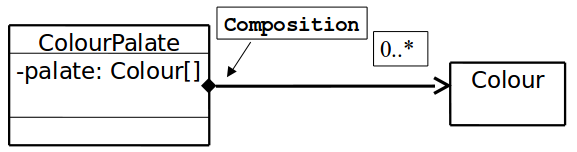
\includegraphics[scale=0.3]{staticUML.png} 
\end{frame}
%--------------------------------------------------------
\defverbatim[colored]\innerClass{
\begin{lstlisting}[style = customjava,basicstyle=\tiny]
public class Outer {
	NestedClass field; // Can have inner class as a field
	int a,b;
	public void aMethod() {
		this.field = new InnerClass(); // Can be declared in a normal method
		InnerClass local = new InnerClass(); // Also fine
	}
	public static void aStaticMethod() {
		InnerClass local = new InnerClass(); // Cannot be instantiated here.
	}
	public static class InnerClass{
		public int add() {
			return a + b; // Uses a and b from Outer		
		}
	}
}

// If public, they can be instantiated outside of the class, but must be associated
// with an Outer object like this:
Outer out = new Outer();
Outer.InnerClass in = out.new InnerClass();
\end{lstlisting}
}
\section{Non-Static Nested Classes}
\begin{frame}
\frametitle{Non-Static Nested Classes}
\begin{itemize}
\item Non-Static Nested Classes are often referred to as {\color{green} inner classes}.
\item They are always associated with an instance of the outer class, they {\color{red} cannot} exist in {\color{red} isolation}.
\innerClass
\end{itemize}
\end{frame}
%-----------------------------------------------------------------
\defverbatim[colored]\interface{
\begin{lstlisting}[style = customjava,basicstyle=\tiny]
Outer out = new Outer();
SomeInterface in = out.factoryMethod();
\end{lstlisting}
}
\subsection{Using Inner Classes}
\begin{frame}
\frametitle{Using Inner Classes}
\begin{itemize}
\item Inner Classes should only be used outside of the top-level class if they implement an interface.
\interface
\item Using an interface like this is a common pattern. The returned object performs some task on the outer object it is associated with.
\end{itemize}
\end{frame}
%----------------------------------------------------------------
\defverbatim[colored]\innerEx{
\begin{lstlisting}[style = customjava,basicstyle=\tiny]
public class TeachingUnit {
	Student[] s;
	StudentStats stats=new StudentStats();

		
	private class StudentStats{
	double maxMark;
	public void findStats(){
		maxMark=s[0].getUnitMark();
		for(int i=1;i<s.length;i++){
			double x=s[i].getUnitMark();
			if(x>maxMark)
				maxMark=x;
	}
	public double getMax(){return stats.maxMark;}
}
\end{lstlisting}
}
\subsection{Inner Class Example}
\begin{frame}
\frametitle{Inner Class Example}
\innerEx
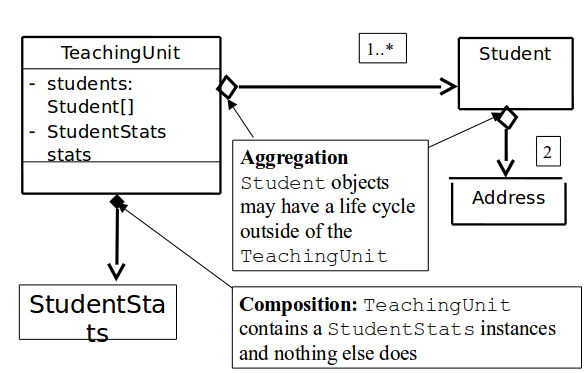
\includegraphics[scale=0.3]{innerUML.png} 
\end{frame}
%------------------------------------------------------------------------
\defverbatim[colored]\local{
\begin{lstlisting}[style = customjava,basicstyle=\tiny]
public void someMethod() {
	class LocalInner{
		...	
	}
	LocalInner in1 = new LocalInner();
	LocalInner in2 = new LocalInner();
}
\end{lstlisting}
}
\section{Local Inner Classes}
\begin{frame}
\frametitle{Local Inner Classes}
\begin{itemize}
\item Defined within a method
\item Multiple instances can be created, but only within the method the class is defined.
\item Barely ever used.
\local
\end{itemize}
\end{frame}
%----------------------------------------------------------------------------------
\defverbatim[colored]\anon{
\begin{lstlisting}[style = customjava,basicstyle=\tiny]
public void someMethod() {
	SomeInterface s = new SomeInterface(){
		public int interfaceMethod(){return 0;}
	};
}
\end{lstlisting}
}
\defverbatim[colored]\anonTwo{
\begin{lstlisting}[style = customjava,basicstyle=\tiny]
JButton button= new JButton("My Button"); 
	button.addActionListener(new ActionListener(){ 
		public void actionPerformed(ActionEvent e){ 
	//do stuff do here
	}
};


new Thread(
	new Runnable() { 
		public void run() 
		{ // do stuff 
		} 
	}
).start();
\end{lstlisting}
}
\section{Anonymous Inner Classes}
\begin{frame}
\frametitle{Anonymous Inner Classes}
\begin{itemize}
\item Defined within a method but can only be created {\color{red} once}.
\item Almost always a throwaway instantiation of an interface.
\anon
\item Often used in swing and Threaded applications.
\anonTwo
\end{itemize}
\end{frame}
%-----------------------------------------------------------------

\defverbatim[colored]\inheritance{
\begin{lstlisting}[style = customjava,basicstyle=\tiny]
public class BaseClass {
   int anInt;
   InnerBase ib1 = new InnerBase();
   protected class InnerBase{ protected double x;}
}
----------------------------------------------------------------------------
public class SubClass extends BaseClass{
  
  InnerBase ib2	 = new InnerBase();
  InnerChild ic1 = new InnerChild();
  
  public class InnerChild extends InnerBase{	  
	public String str;
  }
}
\end{lstlisting}
}

\defverbatim[colored]\inher{
\begin{lstlisting}[style = customjava,basicstyle=\tiny]
SubClass sub=new SubClass();
sub.anInt;
sub.ib1.x;
sub.ib2.x;
sub.ic1.x;
sub.ic1.str;
\end{lstlisting}
}
\section{Inheritance with Nested Classes}
\begin{frame}
\frametitle{Inheritance with Nested Classes}
\begin{itemize}
\item {\color{green} Inner Classes} and {\color{red} Static Nested Classes} can both be extended in a subclass.
\inheritance
\item SubClass has all of the below now:
\inher
\end{itemize}
\end{frame}
%-----------------------------------------------------------------
\section{Summary}
\begin{frame}
\frametitle{Summary}
\begin{itemize}
\item If an instantiation of a class relates to the outer class as a whole and not to a specific \texttt{Object} i.e. It does not need access to fields, use {\color{green}static nested class}.
\item If it needs access to fields, use {\color{red} Non-static inner class}.
\item {\color{brown} Local-Inner classes} and {\color{magenta} Anonymous inner classes} are used to create one off instances of specialised classes.
\item In C++ there is only one type of Nested class and that is the equivalent to Java's {\color{green}static nested class}.
\end{itemize}
\end{frame}
%-----------------------------------------------------------------
\begin{frame}
\Huge{\centerline{The End}}
\end{frame}

\end{document}